\documentclass[11pt, oneside]{article} 
\usepackage{geometry}
\geometry{letterpaper} 
\usepackage{graphicx}
	
\usepackage{amssymb}
\usepackage{amsmath}
\usepackage{parskip}
\usepackage{color}
\usepackage{hyperref}

\graphicspath{{/Users/telliott_admin/Tex/png/}}
% \begin{center} 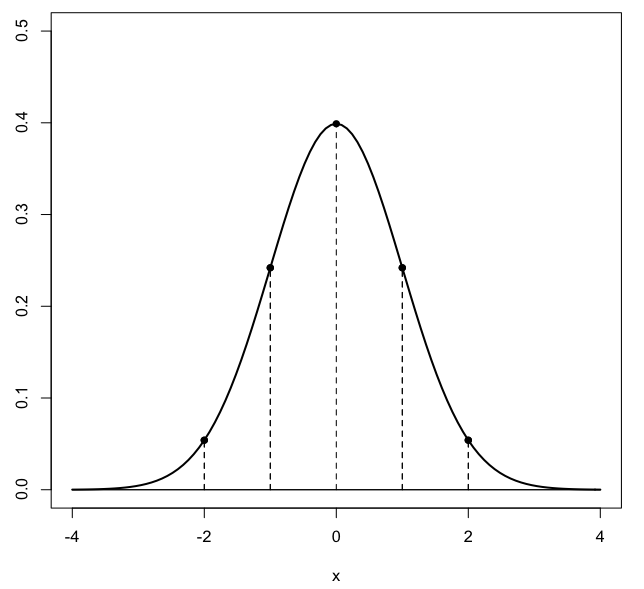
\includegraphics [scale=0.4] {gauss3.png} \end{center}

\title{Relativity and time dilation}
\date{}

\begin{document}
\maketitle
\Large

\subsection*{relative motion}

Imagine that you are seated in a train looking out the window.  Another train is just next to you, sliding past on the adjacent track, moving to your right.

All you can see out the window is the other train and what is happening inside.  This is an idealized world (what Einstein called a Gedanken or thought experiment) so trains do not make noise or lurch from side to side as they move.  

Galileo's classical \textbf{relativity} says that there is no physical test you can do from inside your train to decide which train is moving.  It might be that the other train is moving or it could be that your train is moving.  You can't tell.

\subsection*{vertical and horizontal independence}

\begin{center} 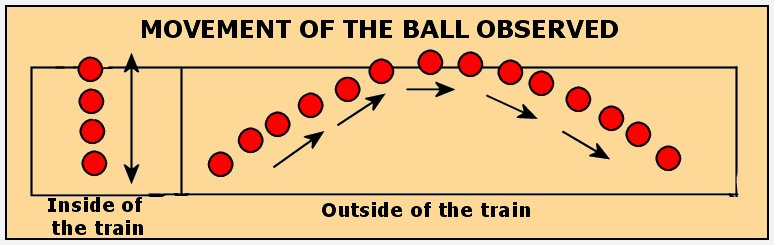
\includegraphics [scale=0.3] {ballmovement.jpg} \end{center}

Suppose there is a guy sitting in the other train and he throws a ball straight up in the air and then it comes down. His view of things is shown on the left, and your view of things is on the right.

You see a horizontal movement that he does not see, because of the relative velocity of the trains.

However, movement in the vertical direction is independent of the horizontal direction and vice-versa, so the time each of you measures for the flight of the ball is the same, governed by its initial velocity upward and the downward force of gravity.  So is the vertical velocity of the ball at each point, and your calculations for the acceleration due to gravity will be the same.

\subsection*{man with a flashlight}

Now suppose instead that the man in the other train is holding a flashlight overhead, pointed at a mirror on the floor.  He turns it on very briefly, emitting a light ray that travels (from his perspective) vertically.  

\begin{center} 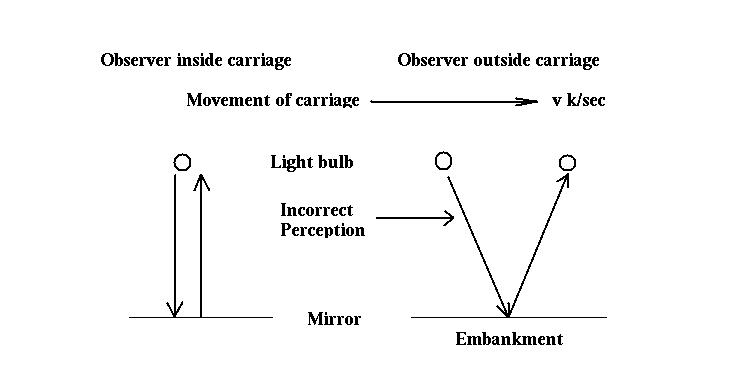
\includegraphics [scale=0.5] {error.jpg} \end{center}

He observes the time when the light returns back from the mirror.  To make things simpler for our calculations, let us just consider the path from the flashlight to the floor.   The light traveled down a distance $e$ in time $s$.

He can calculate the \emph{speed of light} as distance divided by time
\[ c = \frac{e}{s} \]

\subsection*{your view}

Suppose also that the light starts on its journey at precisely the same time as the man, the flashlight and that spot on the floor are all directly opposite you, in your train.

Considered from your perspective, the light ray will cover a longer distance, because of the relative velocity between you and the other train.  

What you see is that the man turned on the flashlight while he was exactly opposite, but by the time the light ray hits the floor, the floor has moved to the right.  So the light travels to the floor by an angled path with distance $d$, hitting the point directly below the other guy when that point is some distance off to your right (it is similar to the example with the thrown ball).

Of course, you must be going very fast for this to be obvious, because the speed of light is so large ($3 \cdot 10^8$ m/sec or about $186,300$ mph).

Suppose that by your watch, the time taken for this to happen is $t$.  $e$ is the vertical component of $d$, and the horizontal component is the relative speed of the two trains $v$ multiplied by your own time $t$.  Speed times time equals distance.

\begin{center} 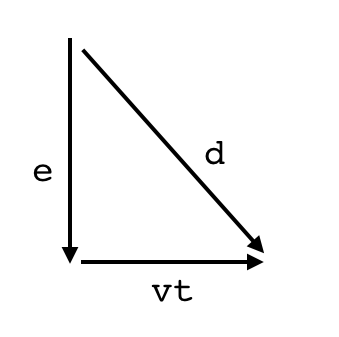
\includegraphics [scale=0.4] {rel_triangle.png} \end{center}

You can also calculate the speed of light.  You saw it move a distance $d$ in a time $t$ so
\[ c = \frac{d}{t}  \]

\subsection*{Einstein's principle of relativity}

One of Einstein's fundamental principles of relativity is that \emph{the speed of light is the same for all observers}.  

We must both obtain the \emph{same} velocity for light:
\[ c = \frac{e}{s} = \frac{d}{t}  \]

Since the distances are clearly not equal ($d \ne e$), neither can the times be equal:  $s \ne t$.  

That is a basic paradox of relativity.  There is no longer such a thing as absolute time.  And if two observers who are in relative motion cannot agree on the time, they will not be able to agree on whether two events are simultaneous or not.

\subsection*{calculation}
A little algebra remains.

We can rearrange what's above above slightly
\[ e = cs, \ \ \ d = ct \]
Since $d$ is the hypotenuse of a right triangle with sides $e$ and $vt$

\begin{center} 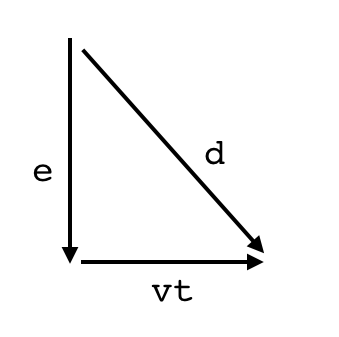
\includegraphics [scale=0.4] {rel_triangle.png} \end{center}
 
Pythagoras tells us that
\[ d^2 = e^2 + (vt)^2 \]
Substitute $d = ct$ and $e = cs$:
\[ (ct)^2 = (cs)^2 + (vt)^2 \]
Isolate the terms containing $t$:
\[ (ct)^2 - (vt)^2 = (cs)^2 \]
Factor out $t^2$
\[ [ \ c^2 - v^2 \ ] \  t^2 = c^2 s^2 \]
Divide by $c^2$
\[ [ \ \frac{c^2 - v^2}{c^2}  \ ] \   t^2 = s^2 \]
\[  [ \ 1 - \frac{v^2}{c^2} \ ] \ t^2 = s^2 \]
\[ \sqrt{1 - \frac{v^2}{c^2}} \cdot t = s \]

Define 
\[ \gamma = \sqrt{1 - \frac{v^2}{c^2}} \]
so
\[ \gamma \ t = s \]

The factor $\gamma$ shows up often in relativity.  

Look again
\[ \gamma = \sqrt{1 - \frac{v^2}{c^2}} \]

If $v = 0$ then $\gamma = 1$, so nothing really changes if the other train is not moving.

As $v$ gets larger, $v^2/c^2$ is always positive so we have the square root of something smaller than $1$, and thus $\gamma < 1$.

Since 
\[ \gamma \ t = s \]
and $\gamma < 1$, it must be that $s < t$.

\emph{The moving observer's value for time, $s$, is smaller than what you measure}, $t$.

If $v$ gets larger, $\gamma$ gets smaller.  

If $v$ were to become as large as $c$, then $\gamma \rightarrow 0$, and then, time would stand still.

\end{document}